\chapter{Implémentation}
    Le projet est développé en c++ utilisant des notions de programmation modernes.
    Un fichier \textit{stdafx.h} était utilisé. Ce fichier avait pour but de centraliser l'intégralité des fichiers d'en tête du projet. Il était ensuite inclus dans tous les fichiers sources. Ce système permet de précompiler les fichiers d'en-tête. Après discussion avec le client, cette fonctionnalité a été enlevée.

    \section{Implémentation générale}
    \subsection{Problème rencontré}
    Le contexte OpenGL créé par le développeur d'origine du projet était faux. Ça se traduisait au niveau
    de l'application par un plantage d'OpengGL sur certaines cartes graphiques. En particulier sur les processeurs graphiques intégrés. Cette erreur a été très vite corrigée.
   
    \subsection{Portage vers \textit{CMake}}
    Le système de compilation du projet repris était basé sur GENie\footnote{\url{https://github.com/bkaradzic/GENie}}, un
    logiciel de configuration utilisant des scripts Lua pour décrire la
    structure du projet, ses dépendances etc. CMake est aussi un logiciel de
    configuration, cependant les scripts de configurations sont écrits dans
    un langage créé pour CMake. Le script de configuration initiale étant
    totalement incompatible, nous sommes repartis de zéro pour la
    configuration de CMake. CMake nous a permis d'inclure le téléchargement
    et la compilation de certaines dépendances à l'étape de compilation,
    simplifiant le déploiement du projet en réduisant le nombre de
    dépendances qui doivent être déjà disponibles sur la cible.
    
    \section{Heightmap}
    Comme expliqué dans le chapitre architecture, la \emph{heightmap} est envoyée sur la carte graphique sous la forme
    d'une texture.\\
    Dans la version de base du projet, seules des \emph{heightmaps} sont chargées depuis le disque. Ces images codées sur un
    seul octet signé sont alors converties en flottant et envoyées à la carte graphique. Cette implémentation pose un très gros problème de précision des valeurs, ces dernières entant comprise entre 0 et 255 ne sont pas suffisantes pour représenter
    avec précision une hauteur. C'est-à-dire que la carte de hauteur sera appliquée sur la planète entière mais dès que l'on va zoomer, les valeurs ne seront pas suffisante pour placer avec précision le sommet.
    
    \subsection{Implémentation de base}
    Pour résoudre ce problème, le programme de base charge quatre autres cartes de hauteur avec des niveaux de détails plus élevés. Cependant, cette implémentation créée d'autres problèmes, le plus important est que les différentes textures détaillées nommées \textit{MoonDetail1}, \textit{MoonDetail2} et \textit{MoonHeightDetail1} sont chargées depuis le disque dans le constructeur de la classe Planet. Ce qui casse l'architecture globale du projet, la classe Planet étant une classe abstraite qui se dérive en différents types de planètes tels que Moon ou Earth.
    Cela implique que lorsque la planète terre est créée, les textures détaillées de la lune sont chargées et appliquées.
    Visuellement cela se traduit par l'affichage des cratères de la lune sur la terre.

    L'utilisation des cartes de hauteurs de différents niveaux de détails pose aussi un problème de discontinuité dans le plaquage des textures qui se traduit par des sauts importants dans les hauteurs affichées.\\
     
    \begin{figure}
        \centering
        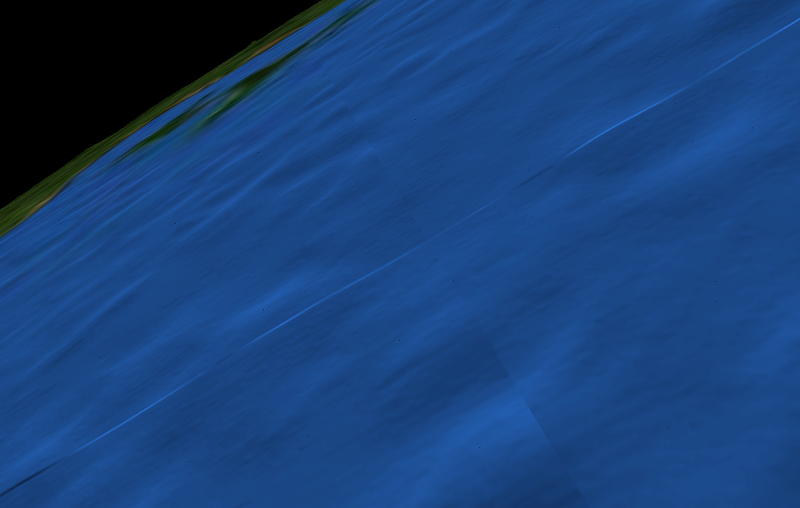
\includegraphics[width=12cm]{img/earth2.png}
        \caption{Affichage de la terre (contraste augmenté)}
        \label{fig:earth}
    \end{figure}
    
    
    La figure \ref{fig:earth} présente les deux problèmes majeurs, on peut voir dans l'océan les cratères induits par la texture de la lune. On peut aussi remarquer au centre de l'image une discontinuité.\\
    
    \paragraph{Critique} On peut aussi critiquer l'utilisation de textures chargées depuis le disque car ces dernières, à l'instar d'une génération procédurale passée par des prétraitements et des formats de fichiers avec compression.
    %\textbf{TODO : Peut être éclaicir l'image pour mieux distinger les artéfacts}
    
    \begin{figure}
        \centering
        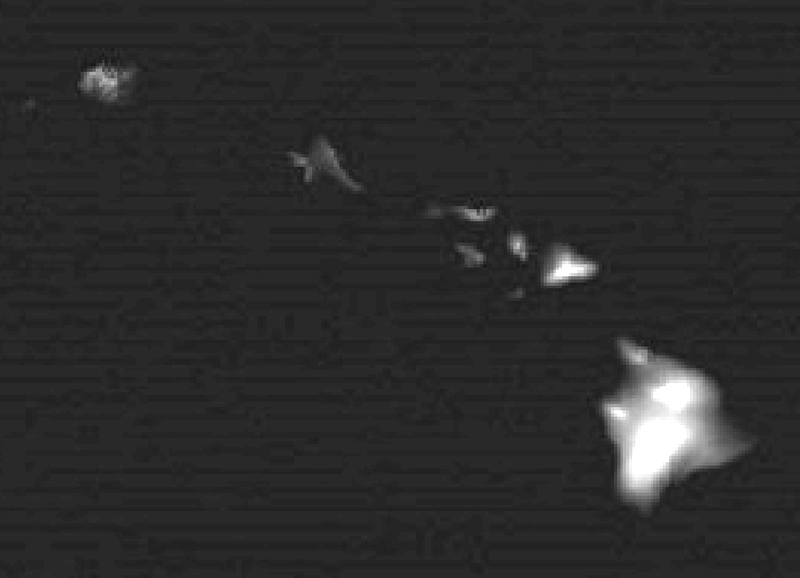
\includegraphics[width=12cm]{img/hawaii2.png}
        \caption{Archipel d'Hawaii (contraste augmenté)}
        \label{fig:hawaii}
    \end{figure}
    
    La figure \ref{fig:hawaii} représente l'archipel d'Hawaii extrait de la carte de hauteur de la terre
    (\textit{EarthHeight16k.jpg}). On distingue très clairement des artéfacts dans la partie océan.
    
    \subsection{Travail effectué}
    Une classe \emph{Procedural} a été écrite, elle permet de créer une planète en utilisant un algorithme de bruit
    sur la texture de la carte de hauteur.
    Des modifications importantes ont été faites dans le code de Texture et dans le \emph{shader patch}.
    Un nouveau constructeur a été écrit pour prendre en charge ce nouveau type de texture. En effet de 
    base le constructeur reçoit une chaîne de caractères représentant un chemin d'accès sur le disque.
    Ce nouveau constructeur prend quand à lui un tableau à deux dimensions de flottants et sa taille en paramètre.\\
    La méthode $Texture::load$ a aussi été modifiée pour permettre l'envoi de ce tableau directement à la carte graphique.\\
    
    \subsection{Correction des problèmes}
    Le problème subsiste lorsque qu'on charge une image depuis le disque mais lorsque l'on génère procéduralement une image,
    il n'y a pas de conversion vers des nombres flottants donc le problème ne se pose pas. Les données sont directement des flottants dispersés sur toute la gamme [-1;1].\\
    De même, comme des données suffisamment précises sont créées, il n'est plus nécessaire de charger des images supplémentaires. Ce qui corrige aussi les problèmes de discontinuités.\\
    L'image doit cependant être générée avec un algorithme de bruit 3d.\\
    
    Un bug a longtemps subsisté, un dépassement de tampon au sein des pilotes graphiques. 
    Les données pointées lors de ce dépassement étant indéfinis, certains sommets pouvaient avoir une hauteur bien supérieure à la normal. Une solution provisoire était de seuiller les sommets dans le \textit{shader}.\\
    Finalement la solution a été trouvée, le problème était qu'un tableau à deux dimensions était alloué.
    Bien que la fonction d'OpenGL requière une hauteur et une largeur, il faut lui passer un tableau à une dimension. Une explication plus détaillée est faite dans la section \ref{sec:class_texture}
    
   \section{Génération du maillage}	% Explication de triangulator.
   La génération du maillage est réalisée en 2 parties distinctes: La première s'éffectue sur le CPU, la seconde sur le GPU. Les classes directement concernées sont Triangulator et Patch.
  % icosaèdre ?
  % triangulator ?
  % structure de données
  \subsection{Triangulator}
	\subsubsection{Icosaèdre}
	\label{subsec:icosaèdre}
	
	La génération du maillage est récursive et s'effectue sur des triangles. A l'initialisation, il faut donc une figure géométrique composée de triangle et approchant le plus possible une sphère. L'auteur a choisit l'Icosaèdre. Ce polyèdre est composée de douze sommets de base et de vingt faces. Chaque face étant un triangle équilatéral de taille identique.
	
	Pour se faire il est nécessaire d'utiliser le nombre d'or $\Phi = \frac{(1+\sqrt(5)}{2}$ , qui est le seul rapport permettant de construire le plus petit deltaèdre ( polyèdre dont les faces sont toutes des triangles équilatéraux).
	
	La méthode utilisée pour former les triangles équilatéraux (et donc l'icosaèdre) et de se servir de 3 plans respectant les proportions du nombre d'or, qui se coupe en leur centre. En reliant les 12 sommets possibles, on va ainsi former les 20 faces de notre icosaèdre, comme on peut l'observer sur la figure \ref{fig:plans-icosaèdre}.
	
	\begin{figure}[H]
        \centerline{
            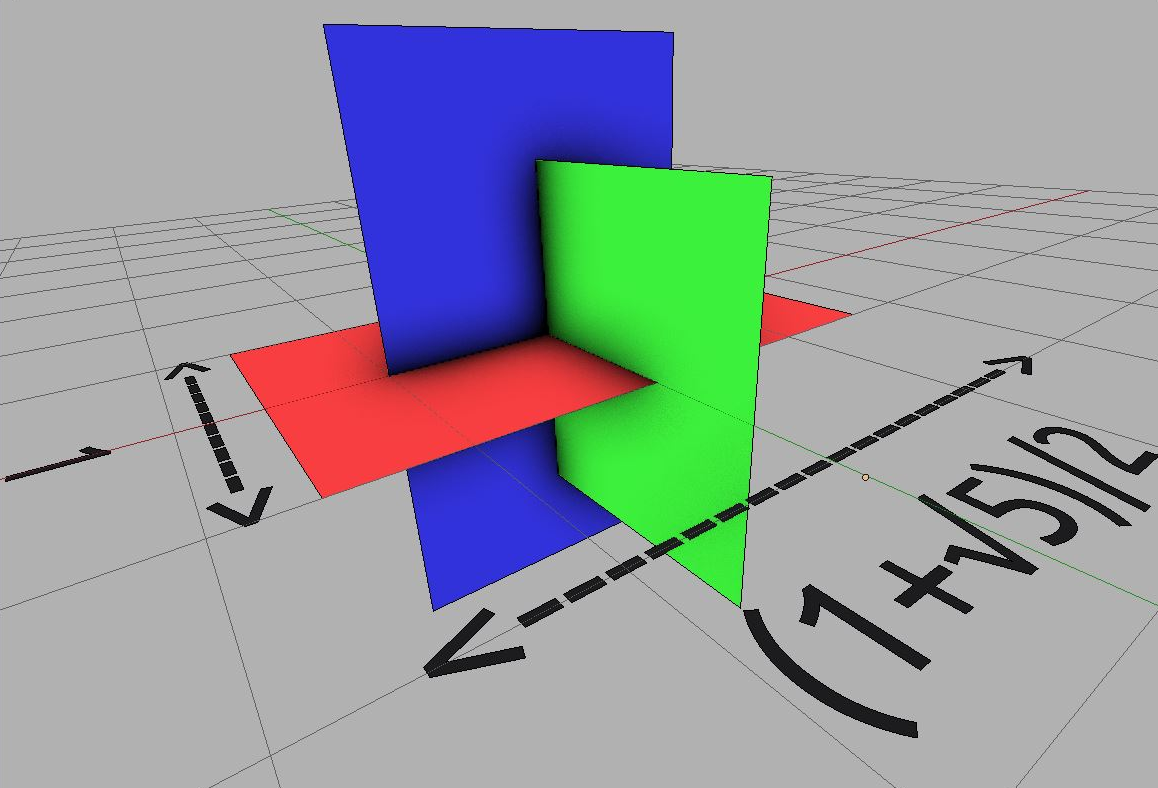
\includegraphics[height=4cm,width=4.5cm]{img/3plans.png}
            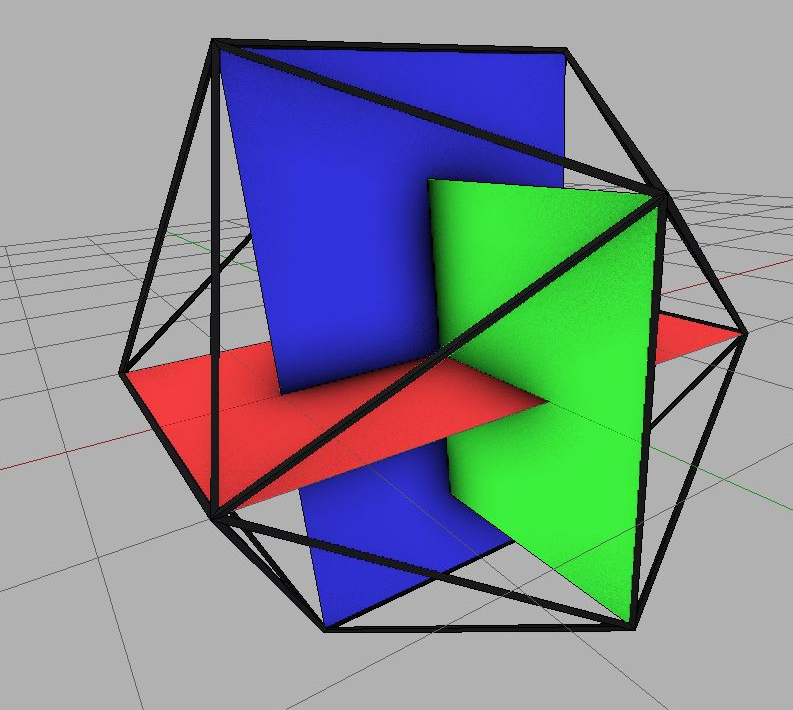
\includegraphics[height=4cm,width=4cm]{img/3plans2.png}}
        \caption{Formation de l'icosaèdre \protect\footnotemark}
        \label{fig:plans-icosaèdre}
	\end{figure}
	\footnotetext{Extrait de \url{http://robert-lindner.com/img/blog/planet_renderer/week5-6/researchPaper.pdf}, dernier accès Mars 2018}
	
	
	% Parler de la generation avec le nombre d'or
	\subsubsection{Récursion}
	
	La récursion prend en entrée un triangle et un booléen spécifiant s'il faut faire un test de frustum culling (toujours vrai au début). Pour chaque triangle, elle s'appuie sur SplitHeuristic() pour savoir si elle doit :
	\begin{itemize} 
	\item le dessiner (LEAF)
	\item l'éliminer (CULL)
	\item le subdiviser (SPLITCULL)
	\item le subdiviser sans faire attention au frustum culling (SPLIT)
	\end{itemize}
	\paragraph{}
	Chacun des cas est expliqué dans la section \ref{sec:SplitHeuristic}. 
	La distinction entre le cas 3 et 4 est nécessaire pour des raisons de performance. Pour beaucoup de triangles (au centre de la caméra), on peut se rendre compte dès le premier niveau que tous les fils sont dans le frustum (plus de détails dans la section \ref{sec:Frustum}).Ainsi, sur une telle branche de la récursion, il ne sert à rien de réexaminer en permanence l'intersection avec le frustum. D'autant plus que selon valgrind, cet examen est coûteux (voir annexe \ref{fig:perfCulling}).
	
	\begin{figure}[H]
        \centerline{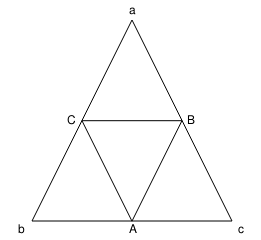
\includegraphics[width=5cm]{img/TriangleSplit.png}}
        \caption{Division}
        \label{fig:TriangleSplit}
    \end{figure}
    Pour subdiviser un triangle abc, on commence par calculer les 3 milieux A B C.
	 On peut ensuite continuer la récursion sur les triangles aBC, AbC, ABc et ABC.
	
\iffalse
L'arbre de données est implémenté avec la méthode des flux du CDLOD (StreamingCDLOD), dont les avantages ont été expliqué précédemment.
	L'implémentation ici ne suit pas entièrement le standard du \textit{StreamingLOD}, il a été expliqué que l'algorithme peut conserver les parties qui restent dans le champ de vision. Ici l'intégralité de l'arbre est régénéré à chaque tour de boucle. Cependant dans un contexte de visualisation simple les gains de performances engendrés par de telles optimisations sont négligeables.
	
	Pour accélérer les temps d'accès mémoire, les distances avec les différents triangles sont conservées
	dans un tableau. \\

	Dans l'arbre, chaque n\oe{}ud possède trois positions correspondant aux trois points du triangle,
	ainsi que quatre pointeurs vers les niveaux suivants.
	D'autres informations sont stockées comme un pointeur vers son parent, le niveau actuel du
	n\oe{}ud dans l'arbre ou encore un drapeau correspondant au type du n\oe{}ud.
	Le drapeau sous forme d'un \emph{enum} permet de distinguer le n\oe{}ud qui sont a l'intérieur de l'arbre de ceux
	qui ne le sont pas. Il permet aussi de renseigner si le n\oe{}ud est une feuille.
		
	Pour chaque triangle, on commence par tester si le triangle est visible, c'est-à-dire s'il est
	présent à l'intérieur du cône de vision de la caméra. Si c'est le cas, on prend le centre de chaque
	arrête du triangle l'on recommence de manière récursive tans qu'une subdivision est nécessaire.
	C'est-à-dire tans que le n\oe{}ud contenant le triangle n'est pas une feuille. Dans le cas contraire,
	\fi	
	
	
    
	
	
	
	\subsubsection{SplitHeuristic}
	\label{sec:SplitHeuristic}
	La méthode SplitHeuristic, associée aux différentes tables LUT, prend un triangle et retourne :
	\begin{itemize} 
	\item CULL: 
	 \newline si le triangle ne fait pas face à la bonne direction, (Backface Culling) ou si aucun triangle de la descendance n'est dans le frustum(cf: section Frustum \ref{sec:Frustum}).
	\item LEAF: 
	\newline si le triangle est suffisamment détaillé par rapport à sa distance à la caméra.
	\item SPLIT: 
	\newline si la totalité de la descendance est dans le frustum, ou que le mode Frustum culling est désactivé.
	\item SPLITCULL:
	\newline si aucune des situations précédentes ne s'appliquent.
	\end{itemize}
	 
	

	
	
	\subsection{Patch}
	\subsubsection{Découpe d'un Triangle}
	La classe Patch met en place le mécanisme de subdivision des triangles envoyés par Triangulator. On parle cette fois-ci de grosse subdivision. La figure \ref{subfig:morph5} montre un découpage avec un nombre de points sur la base (RC) valant 5 (à l'étape \ref{subfig:morph1}, vous pouvez voir 5 points sur la base). Au cours d'un lancement normal, RC vaut 17.\\
	Pour créer la découpe, l'auteur procède comme suit:
	\paragraph{}
	On se place dans un système de coordonnées en deux dimensions correspondant au repère formé par le point inférieur gauche du triangle, et des 2 vecteurs correspondant aux 2 autres points du triangle équilatéral de la petite division(le petit triangle en bas à gauche de l'étape \ref{subfig:morph1}).
	\paragraph{}
	On itère sur les points en partant de la base, de gauche à droite, puis étage par étage. Ainsi à chaque itération, en mémorisant l'étage et la position dans l'étage, on obtient directement les coordonnées du point dans le repaire indiqué. Cette coordonnée permettra à la carte graphique de savoir où placer le point.
	\paragraph{}
	Reste à lui indiquer la direction que devra prendre le point lors du morphing. 
	Cette direction doit provoquer une rotation harmonieuse des points, et faire en sorte que les triangles vers le bas continuent de partager leurs points avec les autres. Ce n'est pas évident à voir, mais cela dépend uniquement de la parité des coordonnées. 
	\paragraph{}
	Il ne reste plus qu'à préciser au GPU à quels points il faut "se lier" pour former les micros-triangles. Cela ce fait, dans le contexte OpenGl, en remplissant un buffer d'indice décrivant l'ordre dans lesquelles les VAO seront envoyés au pipeline graphique. Il faut, pour chaque point, envoyer son indice, l'indice de son voisin du haut, et l' indice du voisin de droite.%todo je maîtrise pas du tout cette partie, alors si quelqu'un a le bon vocab et surtout a déjà utilisé les VAO VBO EBO indexé, qu'il hésite pas.
	\paragraph{}
	Une fois dans le shader, la carte graphique connaît donc le point et la direction du morph. Elle connaît aussi la table des distances. Pour connaître l'intensité du morph à appliquer, elle regarde dans quelle mesure le point était proche de passer aux niveaux suivants. Plus il était proche, plus le point décalé dans la direction de son morph.
	
	
  \subsubsection{Application du morphing}
  La figure \ref{fig:morphTri} représente les déformations causées par le \textit{morphing} lors du rapprochement de la caméra. Le fonctionnement reste assez semblable à celui expliqué dans la section morphing \ref{subsec:morphing} mais est ici appliqué sur des triangles.
  	
\begin{figure}[H]
    \centering
    \begin{subfigure}[b]{0.17\textwidth}
       \centering 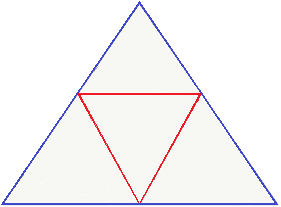
\includegraphics[width=\textwidth,height=2.25cm]{img/morph5.png}
       \caption{}\label{subfig:morph5}
    \end{subfigure}
    ~ 
    \begin{subfigure}[b]{0.17\textwidth}
       \centering 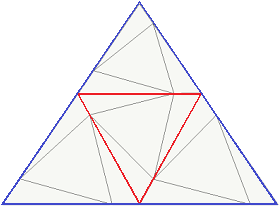
\includegraphics[width=\textwidth,height=2.3cm]{img/morph4.png}
       \caption{}\label{subfig:morph4}
    \end{subfigure}
    ~
    \begin{subfigure}[b]{0.17\textwidth}
       \centering 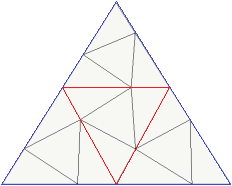
\includegraphics[width=\textwidth,height=2.3cm]{img/morph3.png}
       \caption{}\label{subfig:morph3}
    \end{subfigure}
    ~
    \begin{subfigure}[b]{0.16\textwidth}
       \centering 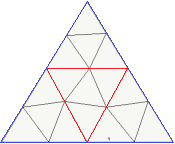
\includegraphics[width=\textwidth,height=2.3cm]{img/morph2.png}
       \caption{}\label{subfig:morph2}
    \end{subfigure}
     ~
    \begin{subfigure}[b]{0.16\textwidth}
       \centering 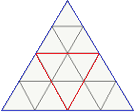
\includegraphics[width=\textwidth,height=2.3cm]{img/morph1.png}
       \caption{}\label{subfig:morph1}
    \end{subfigure}
    \caption{Morph sur des triangles}\label{fig:morphTri}
\end{figure}

    Dans la figure \ref{fig:morphTri}, on représente le découpage d'un triangle du Triangulator, au fur et à mesure que la caméra s'en rapproche. Pour des raisons de simplicité, on prend un découpage très faible.
    Sur la figure \ref{subfig:morph5} le triangle n'est pas encore suffisamment proche pour être déformé. Cependant tous les points (et triangles) dans les autres figures sont présents et dessinés. 
    Lorsque la distance commence à dépasser une certaine limite, les points commencent à divergés vers les directions calculées à l'initialisation. Plus le triangle se rapproche, et plus les points diverges fortement, jusqu'à la figure \ref{subfig:morph1}. Il faut comprendre qu'à la figure \ref{subfig:morph1}, ce n'est plus le même triangle que dans les autres figures, mais le fils du milieu dans la récursion de Triangulator.
    Le morphing est plus important qu'il n'y paraît. Il ne permet pas seulement d'avoir des transitions plus continues en matière de détail. C'est la seule chose qui masque les "trous" à la frontière entre deux zones de niveaux différents comme on peut le voir sur la figure \ref{fig:noMorphingHole}
 \begin{figure}[H]
  \centerline{
  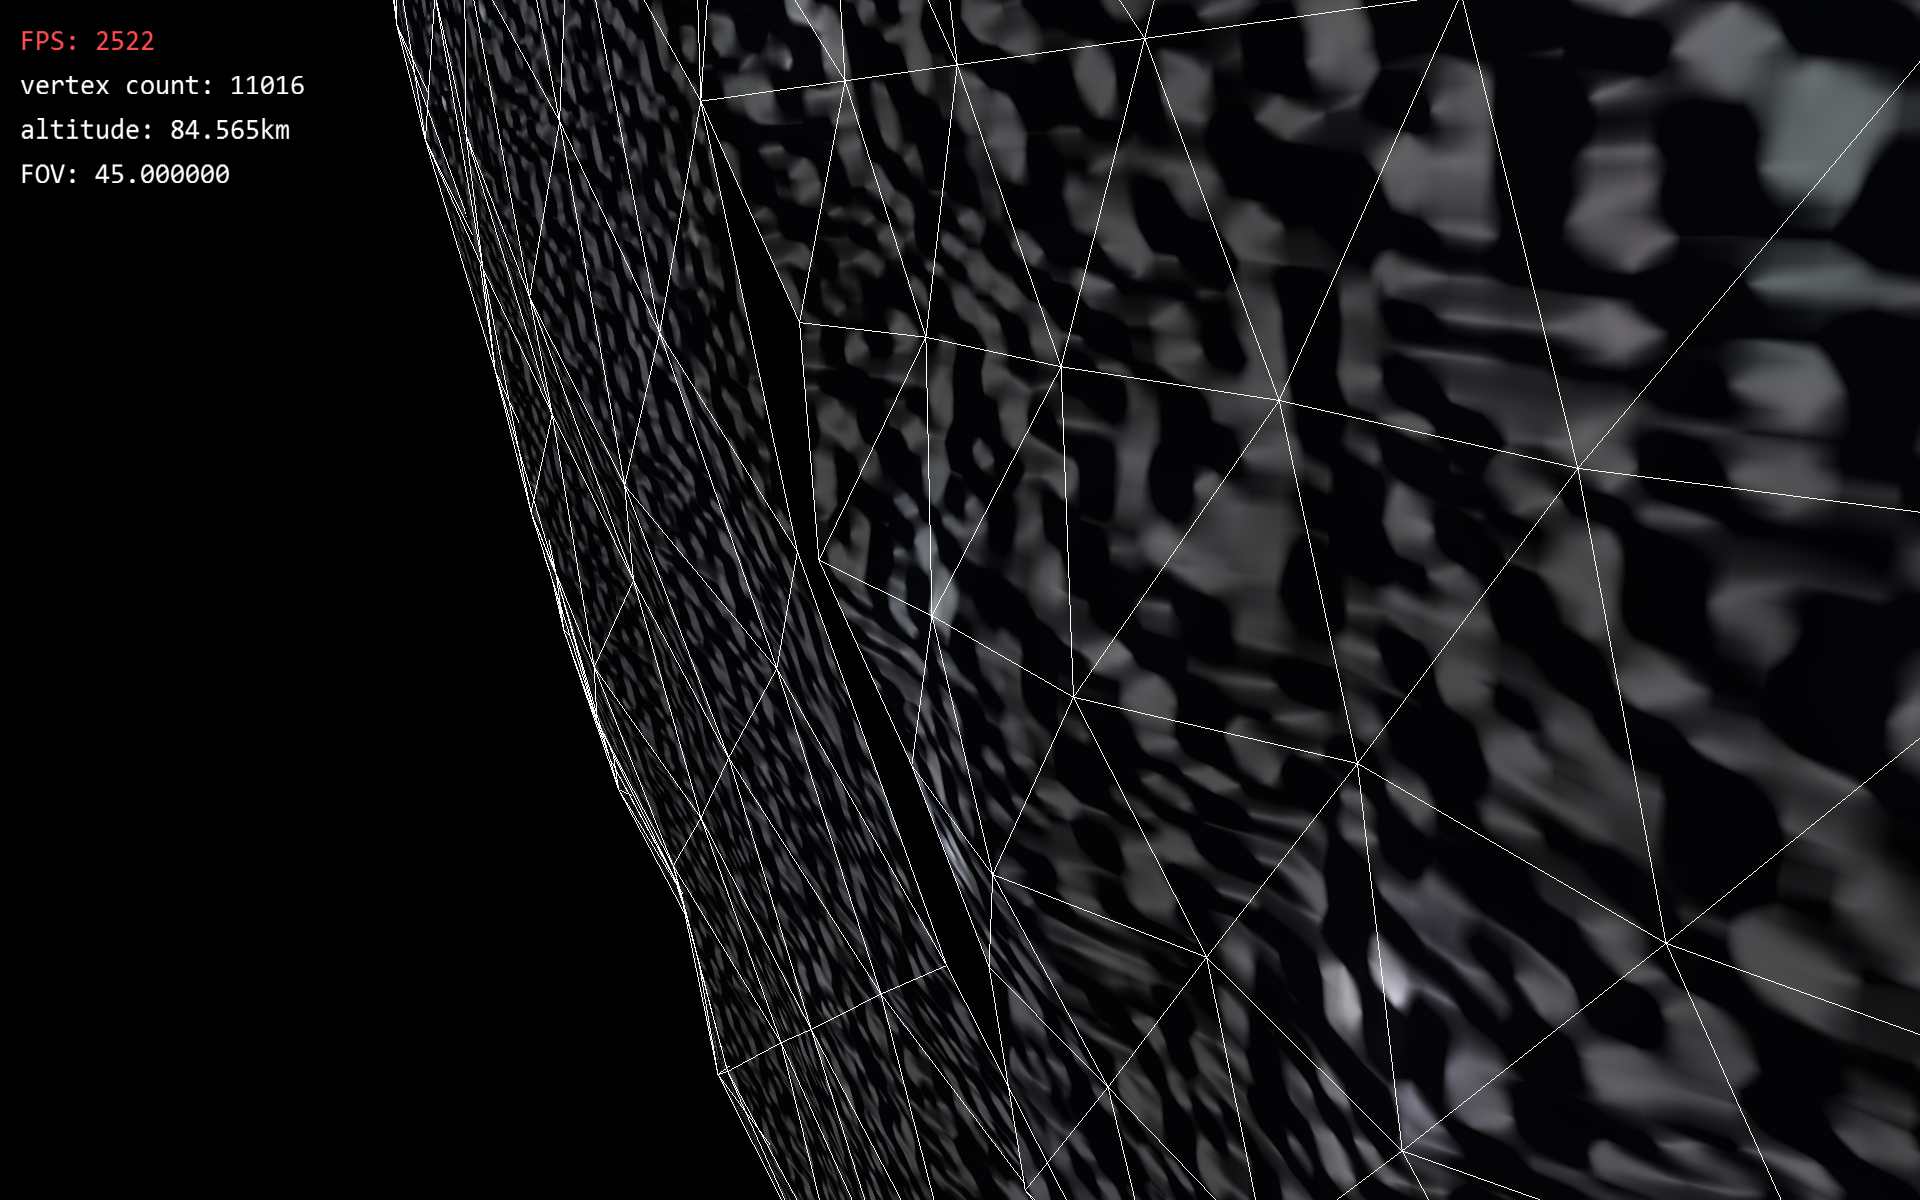
\includegraphics[width=10cm]{img/noMorphingHole.png}}
  \caption{Rendu avec morph désactivé}
  \label{fig:noMorphingHole}
  \end{figure}

  
  \section{Frustum}
  \label{sec:Frustum}
  \begin{figure}[H]
  \centerline{
  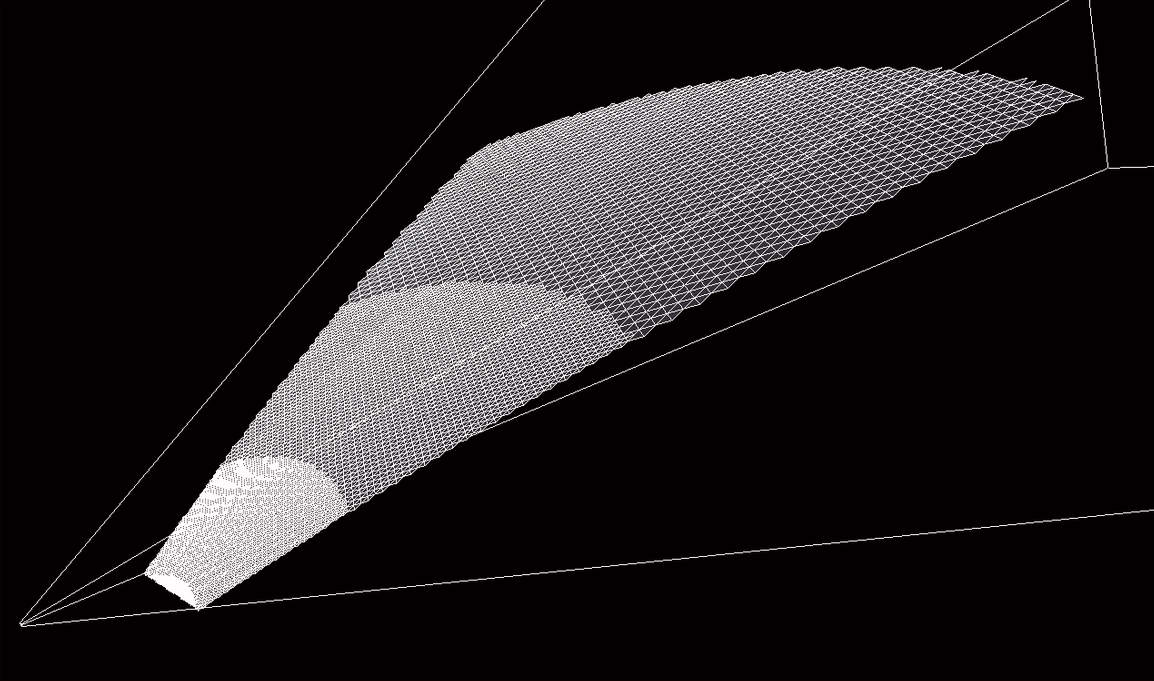
\includegraphics[width=6cm,height=4.5cm]{img/culling.png}
  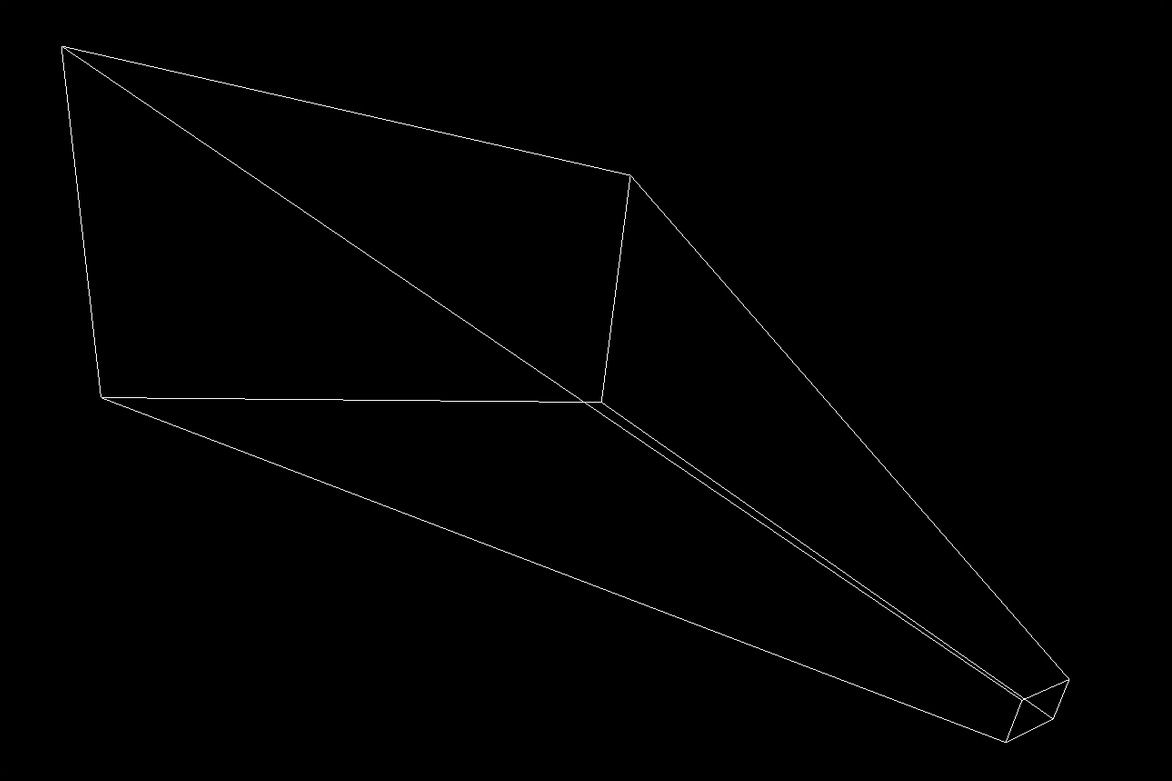
\includegraphics[width=6cm,height=4.5cm]{img/frustumbox.png}}
  \caption{Cône de vision de la caméra \protect\footnotemark}
  \label{fig:culling}
  \end{figure}
  
  Le \textit{frustum} représente la sous-partie de l'espace contenue dans le champ de la caméra. On s'intéresse à cet espace car il permet de ne pas perdre de temps à afficher des triangles hors champs.
  
  

  \footnotetext{Extrait de \url{http://robert-lindner.com/img/blog/planet_renderer/week5-6/researchPaper.pdf}, dernier accès avril 2018}
 
  Le \emph{frustum} est entièrement déterminé par les paramètres de la caméra.  
  En effet, grâce au \textit{FOV}, à la position, la direction et la distance \emph{near}, on peut créer un rectangle \emph{near}. On créait similairement un rectangle far, parallèle au plan \emph{near}. On caractérise alors le \emph{frustum} par 6 plans, dont on obtient la paramétrisation grâce aux triangles formés par les 8 points des deux rectangles, en prenant garde à orienter les normales des plans vers l'intérieur. Visible sur la figure \ref{fig:culling}.
  
  On dispose ensuite d'une méthode simple pour décider si un point est à l'intérieur du \emph{frustum}: il suffit, pour chaque plan, d'évaluer l'équation du plan en les coordonnées du point. Si le résultat est positif pour chacun des plans, c'est que le point est à l'intérieur.
  
  Grâce à cette primitive, l'auteur implémente une technique pour faire la même chose avec un triangle. Pour chacun des six plans, on regarde combien de points sont du côté extérieur. Si ce nombre est différent de 0 ou 3, on peut déjà affirmer que l'intersection est non nulle. Si il vaut 3, alors on peut affirmer que le triangle est complètement hors du \emph{frustum}. Arriver au dernier plan, si le triangle n'est toujours pas classifié, c'est qu'il est totalement inclus dans le \emph{frustum}.
  
  Cependant, lors de la récursion dans Triangulator, il ne suffit pas de tester que le triangle actuel est hors \emph{frustum}. En effet, les fils sont toujours plus haut que les parents. Ainsi si l'on se place de biais à une faible altitude, il est possible que le \emph{frustum} rase un triangle du premier niveau, mais touche les triangles des niveaux suivants. 
  \textbf{TODO rajouter screen shoot culling non protégé}
  Il faut donc "protéger" les triangles. Pour cela, on va réaliser l'intersection du \emph{frustum}, non pas avec le triangle, mais avec le prisme formé par le triangle, et le triangle normé à une certaine hauteur. Il suffit pour cela de reprendre l'algorithme du triangle, mais en considérant cette fois 6 points.
  En ce qui concerne cette hauteur. Le plus simple est de toujours normaliser le triangle sur l'altitude maximale. L'auteur utilise une technique plus poussée, et fait varier cette hauteur en fonction du niveau.  
  
  \section{Génération de la Heightmap}
  
  Dans le code d'origine, les cartes de hauteur étaient chargées depuis le disque. Nous avons développé un nouveau type de planète héritée de \textit{Planet} qui permet de générer une planète avec plusieurs types de bruits différents.
  
  Le processus de création de la texture de bruit se base sur une structure contenant les différents paramètres du bruit.
  Chaque bruit étant spécifique, certain nécessite plus de paramètre que d'autres, par exemple un bruit de \textit{simplex} classique à besoin uniquement d'une taille alors qu'un bruit
  de simplex de type \textit{flow noise} utilise d'autres paramètres comme par exemple un octave. 
  
  \section{Gestion des arguments}
  Nous avons rajouté un système permettant de récupérer et de traiter les valeurs d'entrées du programme.
  Pour cela a été créé une classe \textit{ArgvParser}. Cette dernière est créée grâce aux variables \textit{argc} et \textit{argv}. 
  Cette classe ne gère pas le fait qu'aucun argument ne soit renseigné en entrée. Il faut au préalable s'assurer que \textit{argc} soit strictement supérieur à 1. Ce que l'on fait dans la fonction \textit{main}.\\
  
  \subsection{Classe ArgvParser}
  
  Le but de la classe \textit{ArgvParser} est de récupérer chaque entré de \textit{argv}, les diviser en deux en fonction du caractère "=" et de stocker les deux chaînes de caractères résultantes dans un tableau dynamique de deux-uplets (\textit{tuple}).\\
  
  Par exemple avec une entrée "--width=100", un deux-uplets contenant "--width" et "100" est créé et est stocké.\\
  Si une entrée ne contient pas de "=", par exemple "--help" un deux-uplets est créé, avec "--help" et "true" comme valeur. La valeur par défaut lorsque l'on ne trouve pas de "=" est "true".
  Un autre système avait été mis en place à l'origine. Le concept était d'utiliser des paramètres optionnels
  avec la classe \textit{optionnal} de la bibliothèque standard mais ce système a été standardisé en \textit{C++17} et n'est pas disponible dans la version que l'on utilise. Un exemple de l'utilisation de ce système est renseigné en annexe, 
  
  Des méthodes \textit{GetCmdInt}, \textit{GetCmdFloat} et \textit{GetCmdBool} permettent ensuite de récupérer les valeurs correspondant aux arguments.
  
  \lstset{language=C++}
  \begin{lstlisting}
     int main(int argc, char** argv){
        if (argc <= 1)  return -1;
        
        ArgvParser argvParser (argc, argv);
        
        unsigned int width = 0;
        argvParser.GetCmdInt<unsigned int>("--width", &width);
     }
  \end{lstlisting}
  
   \subsubsection{GetCmd*}
    Les méthodes \textit{GetCmdInt}, \textit{GetCmdFloat} et \textit{GetCmdBool} permettent de récupérer la valeur définie après le égale et de la stocker respectivement dans un entier, flottant et booléen.\\
    
    La méthode \textit{GetCmdInt} utilise de la généricité pour permettre de choisir entre un entier signé et non signé. L'utilisation des entiers non signés n'est cependant pas utilisée.\\
    
    La méthode \textit{GetCmdInt} fonctionne uniquement si le type générique renseigné est \textit{int} ou \textit{unsigned int}. Cette limitation est renseignée dans la documentation de la méthode.
    
  \subsubsection{Limitation}
    
    La classe \textit{ArgvParser} ne gère pas les cas où l'utilisateur renseigne un chiffre négatif alors que le programme attend un chiffre positif. Par exemple la sélection d'une taille de texture négative
    n'est pas traitée à ce niveau. Mais gérée au niveau de la création de la planète dans la classe \textit{Scene}.
  
  \section{Création de la planète}
  Une classe \textit{ProceduralPlanet} a été écrite, elle permet conjointement avec la classe \textit{Scene} et \textit{Texture} de créer une texture en fonction des arguments d'entrer du programme.
  
  \subsection{Classe Texture}
  \label{sec:class_texture}
  La classe Texture permet de charger une texture depuis le disque, de la lier à \textit{OpenGL} pour l'utiliser dans les \textit{shaders}.\\
  
  Cette classe a été modifiée pour pouvoir accepter un pointeur sur une texture déjà existante. 
  La difficulté est de correctement configurer OpenGL pour envoyer des données correctes. Les données dont des flottants codés sur 32bit (GL\_32F).\\
  Nous utilisons la fonction \textit{glPixelStorei(GL\_UNPACK\_ALIGNMENT, 1)} pour préciser que les données envoyées à OpenGL sont contiguës. D'après le standard OpenGL cette fonction est nécessaire mais 
  nous n'avons pas trouvé de différences selon la valeur renseignée.
  
  \subsection{Classe ProceduralPlanet}
    \label{sec::ProceduralPlanet}
  Une structure \textit{Properties} est définie à l'intérieur de la classe \textit{ProceduralPlanet}. Elle permet de faire passer les différents paramètres que chaque bruit ainsi que les différents paramètres. 
  Elle permet de centraliser les paramètres de chaque bruit et est passée par pointeur au constructeur.
  

  \section{Classe Scene}
  Comme vue dans la partie \ref{sec::ProceduralPlanet}, une structure correspondant au bruit voulu est créé,
  elle est ensuite passé sous forme de pointer à la construction de la planète.\\
  
  Le code de création de la fenêtre était à l'origine dans le constructeur, il a été déplacé dans une méthode dédiée \textit{CreatePlanetFromArgs}. Une méthode \textit{check_value} a aussi été écrite, elle permet de mettre une valeur par défaut dans la variable si cette dernière est égale à une valeur de comparaison. On peut voir que dans l'exemple \ref{fig:code_scene} la création d'une planète avec un bruit \textit{FLOW-NOISE}, un angle de 0.5. Les autres paramètres n'étant pas spécifiés, leur valeur est une valeur par défault précisée dans la structure \textit{ProceduralPlanet::Properties}.
  
  \begin{figure}
    \centering
      \lstset{language=C++}
      \begin{lstlisting}
        ProceduralPlanet::Properties prop;
        prop.noise = ProceduralPlanet::Noise::FLOW_NOISE;
        //...
        prop.angle = 0.5;
        check_value<float>(prop.angle, 0, 0.5);
        
        m_pPlanet = new ProceduralPlanet(&prop);
            
        //...
      \end{lstlisting}    
      \caption{Création de la planète}
      \label{fig:code_scene}
  \end{figure}
  
  
  La planète est créée sans aucune vérification des données, cependant si une exception est levée par le constructeur de \textit{ProceduralPlanet}, et est attrapée \textit{Scene} et le programme dans se termine.\\
  C'est par exemple le cas quand une taille de texture négative est renseigné par l'utilisateur.
  
  \section{Fonctions de bruit}
  
  Pour générer la planète, plusieurs type de bruit ont été proposés. Le bruit de Simplex et de Perlin sont implémenté par la bibliothèque glm. Les autres bruits sont des dérivés de Simplex et sont implémenté dans une bibliothèque nommée \textit{SimplexNoise} (source : \url{https://github.com/simongeilfus/SimplexNoise})
  
  N'étant pas central dans le projet, nous considérons ces fonctions de bruis comme des fonctions boîtes noires.
  Les bruits sont crées grâces à des points en trois dimensions. Pour être appliqué sur une sphère, ce sont des coordonnées polaires qui sont utilisées. Elles sont ensuite converties en coordonnées cartésiennes pour être utilisées sous la forme d'un point 3D.\\

  %TODO expliquer vite fais les bruits
  
%  \section{Calcul de la lumière}
%  \label{sec:phong}
%  \textbf{TODO SI ON A LE TEMPS}